\documentclass{article}

\usepackage{mathtools,amsfonts}
\usepackage{enumitem}
\usepackage{fullpage}
\usepackage{fancyvrb}
\usepackage{hyperref}


\begin{document}
\thispagestyle{empty}

\begin{center}
  \textbf{\Large <LEVEL> Test <NUMBER>}
  % LEVEL is Senior, Intermediate or Beginner
  % NUMBER is the test number: 1, 2, etc.
  \\ \vspace{1em}
  \textbf{\large Stellenbosch Camp 2022}
  \\ \vspace{1em}
  \textbf{\large Time: $2\frac{1}{2}$ hours}
\end{center}

\bigskip

\begin{enumerate}[itemsep=\fill]

\item % Source of problem
Problem statement


\item %
For nonzero real numbers $a$, $b$, and $c$, show that
\[ \frac{a}{b} +\frac{b}{c} +\frac{c}{a} = \frac{a}{c} +\frac{c}{b} +\frac{b}{a} \]
if and only if two of $a$, $b$, and $c$ are equal.

\textbf{Solution:} Observe the following computation:
\begin{align*}
\frac{a^{2}b + b^{2}c + c^{2}a}{abc} & = \frac{a^{2}c + b^{2}a + c^{2}b}{abc}\\
 0 & = \frac{a^{2}c + b^{2}a + c^{2}b -(a^{2}b + b^{2}c + c^{2}a)}{abc} \\
 0 & = \frac{abc + a^{2}c + b^{2}a + c^{2}b - (a^{2}b + b^{2}c + c^{2}a+abc)}{abc} \\
 0 & = \frac{(a-b)(b-c)(c-a)}{abc} \\
\end{align*}
One of $a-b$, $b-c$, $c-a$ must be zero, showing that some pair among $a$, $b$, $c$ must be equal.

\item % Tsimerman
Can you tile a $10\times 10\times 10$ cube with $4\times 1\times 1$ blocks? (Standard tiling rules apply---cover the whole volume, no overlaps, etc.)

\textbf{Solution:} The answer is no. Consider the following colouring: there are 10 `layers' to the cube. Label these layers from 1 to 10. For layers 1,2,5,6,9,10, we colour the layer as follows:
\begin{center}
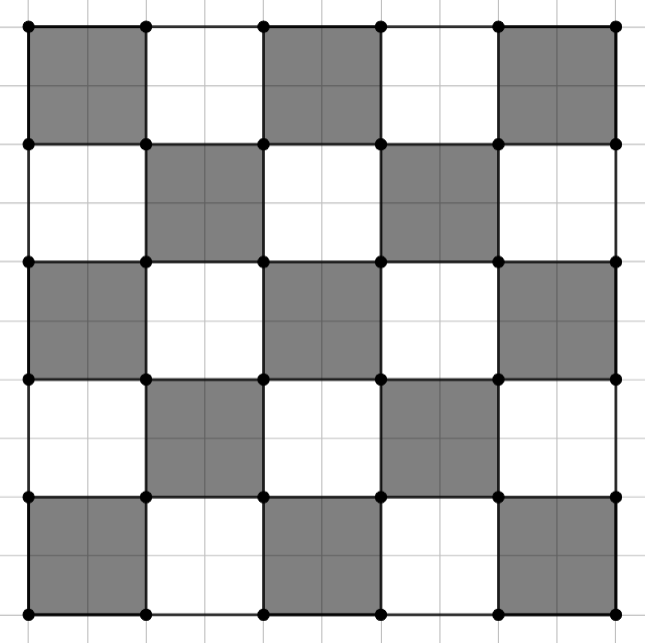
\includegraphics[scale=0.5]{Capture.png}
\end{center}
For layers 3,4,7,8, we invert these colours.\\
We note that each $4\times 1\times 1$ covers exactly 2 shaded blocks and 2 unshaded.\\
But counting the total number of shaded blocks gives 504, while there are 496 unshaded blocks.\\
Thus, we can not tile the shape as requested. 


\item % 
Consider an infinite sequence $(a_n)_{n=0}^{\infty}$ of positive integers such that for $n \geq 0$, we have that
\[
    a_{n + 1} = a_n + b_n
\]
where $b_n$ is the last (units) decimal digit of $a_n$. Show that the sequence contains infinitely many powers of $2$ if and only if $a_0$ is not a multiple of $5$.

\textbf{Solution:} If $a_0$ is a multiple of 5, it will end in a 0 or 5 and be at least as big as 5. $a_1$ will then end in a 0, and the sequence becomes constant.\\
Assume $a_0$ is not a multiple of 5. $a_1$ will end in an even digit. We will now continue to cycle through the last digits $2\rightarrow 4 \rightarrow 8 \rightarrow 6$, whose sum is 20. Thus, we will obtain all numbers of the form $a_1+20k$.\\
We look at the last two digits of $2^n$ and note that they will repeat in the pattern $$\textbf{04}, 08, 16, 32, 64, 28, 56, 12, 24, 48, 96, 92, 84, 68, 36, 72, 44, 88, 76, 52, \textbf{04}, 08, ...$$
If the second last digit of $a_1$ is even and the last digit is 4 or 8, then we will obtain all powers of 2 ending in 4 or 8. If the second last digit is odd and the last digit is 2 or 6, we will obtain all powers of 2 ending in 2 or 6.\\
If $a_1$ ends in a 4, and the second last digit is odd, then $a_4$ will be $a_1+18$, which will end in a 2 and have the second last digit odd. We will now obtain all numbers of the form $a_4+20k$, which again gives infinite powers of 2.\\
If $a_1$ ends in a 8 and the second last digit is odd, then $a_3=a_1+14$ will end in a 2 and the second last digit will be odd. A similar argument applies.\\
If $a_1$ ends in a 2 and the second last digit is even, then $a_2=a_1+2$ ends in a 4 and the second last digit is even.\\
If $a_1$ ends in a 6 and the second last digit is even, then $a_2=a_1+6$ ends in a 2 and the second last digit is odd.


\item % 

\end{enumerate}


% ASCII art
\centering
\small
\begin{BVerbatim}
% Insert art here
\end{BVerbatim}

\end{document}
